\documentclass[times, utf8, zavrsni, numeric]{fer}
\usepackage{booktabs}
\usepackage{listings}
\usepackage{listingsutf8}
\usepackage{float}
\usepackage[T1]{fontenc}
\usepackage[scaled]{beramono}
\usepackage{xcolor}

\definecolor{bluekeywords}{rgb}{0.13,0.13,1}
\definecolor{greencomments}{rgb}{0,0.5,0}
\definecolor{redstrings}{rgb}{0.9,0,0}

\lstdefinestyle{csharp}
{
language=[Sharp]C,
showspaces=false,
showtabs=false,
tabsize=4,
breaklines=true,
showstringspaces=false,
escapeinside={(*@}{@*)},
commentstyle=\color{greencomments},
keywordstyle=\color{bluekeywords}\bfseries,
stringstyle=\color{redstrings},
inputencoding=utf8/latin4,
basicstyle=\fontsize{11}{10}\selectfont\ttfamily
}

\lstdefinestyle{sql}
{
language=SQL,
showspaces=false,
showtabs=false,
tabsize=4,
breaklines=true,
showstringspaces=false,
breakatwhitespace=true,
escapeinside={(*@}{@*)},
commentstyle=\color{greencomments},
keywordstyle=\color{bluekeywords}\bfseries,
stringstyle=\color{redstrings},
inputencoding=utf8/latin4,
basicstyle=\fontsize{11}{10}\selectfont\ttfamily
}

\lstdefinestyle{html}
{
language=html,
showspaces=false,
showtabs=false,
tabsize=4,
breaklines=true,
showstringspaces=false,
breakatwhitespace=true,
escapeinside={(*@}{@*)},
commentstyle=\color{greencomments},
keywordstyle=\color{bluekeywords}\bfseries,
stringstyle=\color{redstrings},
inputencoding=utf8/latin4,
basicstyle=\fontsize{11}{10}\selectfont\ttfamily
}

\lstdefinelanguage{JavaScript}{
  keywords={typeof, new, true, false, catch, function, return, null, catch, switch, var, if, in, while, do, else, case, break},
  keywordstyle=\color{blue}\bfseries,
  ndkeywords={class, export, boolean, throw, implements, import, this},
  ndkeywordstyle=\color{darkgray}\bfseries,
  identifierstyle=\color{black},
  sensitive=false,
  comment=[l]{//},
  morecomment=[s]{/*}{*/},
  commentstyle=\color{purple}\ttfamily,
  stringstyle=\color{red}\ttfamily,
  morestring=[b]',
  morestring=[b]"
}


\lstdefinestyle{js}
{
language=JavaScript,
showspaces=false,
showtabs=false,
tabsize=4,
breaklines=true,
showstringspaces=false,
breakatwhitespace=true,
escapeinside={(*@}{@*)},
commentstyle=\color{greencomments},
keywordstyle=\color{bluekeywords}\bfseries,
stringstyle=\color{redstrings},
inputencoding=utf8/latin4,
basicstyle=\fontsize{11}{10}\selectfont\ttfamily
}

\begin{document}

\thesisnumber{4439}

\title{Baza podataka i Web aplikacija za upravljanje vremenom tijekom studija}

\author{Vedran Biđin}

\maketitle

\textbf{Izvornik}\\\hspace*{\fill}

Oblikovati model baze podataka za praćenje vremena utrošenog na aktivnosti tijekom direktne nastave, učenje i ostale nastavne obaveze studenta tijekom studija. Model treba, između ostalog, obuhvatiti podatke o predmetima i njihovom predviđenom opterećenju izraženom u ECTS bodovima, fiksnim nastavnim obavezama studenta tijekom semestra i stvarno utrošenom vremenu tijekom samostalnog rada studenta. Na osnovi izgrađenog modela implementirati bazu podataka i pripadnu web aplikaciju. Aplikacija treba putem prikladnog sučelja korisniku omogućiti evidentiranje i pregled utrošenog vremena te usporedbu stvarnog utroška vremena s vremenom koje je ECTS bodovima propisano za uspješno savladavanje nastavnih obaveza. Uz otisnuti primjerak rada priložiti optički disk s izgrađenom programskom potporom u izvornom i izvršnom obliku, te tekstom rada.

\zahvala{}

\tableofcontents

\chapter{Uvod}
TODO

\chapter{Baza podataka}

\section{Opis problema}
Web aplikacija mora omogućiti korisnicima, odnosno studentima, da evidentiraju vrijeme koje su utrošili tijekom studija na aktivnosti kao što su direktna nastava, učenje, te ostale nastavne obaveze studenata. Sustav također mora omogućiti korisnicima da pregledavaju utrošeno vrijeme te da uspoređuju stvarno utrošeno vrijeme sa vremenom koje je ECTS bodovima propisano za uspješno svladavanje nastavnih obaveza.

Zadatak stvaranja baze podataka web aplikacije podrazumijeva dizajn sheme baze. Potrebe korisnika igraju središnju ulogu u konstruiranju sheme. Početna faza dizajna baze podrazumijeva opisivanje u potpunosti potrebe potencijalnih korisnika. Ishod ove faze u složenijim aplikacijama može biti specifikacija zahtjeva korisnika. Nakon što su definirani svi zahtjevi, iz njih se izvodi konceptualni model baze podataka.
\begin{enumerate}[leftmargin=*]
\item Svaki korisnik mora moći evidentirati te pregledavati svoje utrošeno vrijeme. Sustav mora razlikovati između različitih korisnika. To se obično postiže tako da svaki korisnik ima na raspolaganju svoj vlastiti korisnički račun, te se sve evidencije koje on provodi implicitno vežu na njegov korisnički račun. Potrebno je implementirati tipični sustav za prijavljivanje, koji omogućuje korisnicima da se prijave na svoj korisnički račun uporabom korisničkog imena i lozinke, ili da naprave novi račun sa svim potrebnim podacima u slučaju ako nemaju već postojeći korisnički račun. Također je korisnicima potrebno omogućiti neke osnovne funkcionalnosti za mijenjanje postojećih korisničih podataka kao što su lozinka, e-mail, i slično.

\item Korisnik mora moći evidentirati svoje utrošeno vrijeme. Evidencija vremena međutim mora biti na neki način vezana uz određenu aktivnost ili nastavnu obavezu. Nema smisla da korisnik samo evidentira utrošeno vrijeme, jer to može značiti da je vrijeme utrošeno na apsolutno bilo koji dio studija, a takve evidencije ne pružaju ikakvu informaciju vrijednu sakupljanja niti pregleda. Dakle, korisnik mora moći na neki (intuitivni) način u sustavu pronaći specifičnu aktivnost za koju želi evidentirati utrošenu vrijeme.

\item Korisniku je potrebno omogućiti pregled svog trenutačnog utrošenog vremena, i to na taj način tako da se može uspoređivati stvarno utrošeno vijeme korisnika sa vremenom koje je propisano ECTS bodovima, semestralnim opterećenjima, ili na bilo koji drugi način. Da bi to bilo moguće, potrebno je aktivnosti koje korisnik može evidentirati podijeliti na neki način u grupe i propisati im određene očekivane iznose utrošenog vremena koje bi one trebale iznositi. Korisnik bi trebao moći vidjeti ne samo koliko je vremena on utrošio na neku aktivnost, a koliko je 'trebao' utrošiti, nego i koliko je vremena utrošio na sve 'pod-aktivnosti' te aktivnosti (pošto neke aktivnosti implicitno obuhvaćaju druge aktivnosti).
\end{enumerate}

Web aplikacija podrazumijeva korištenje baze podataka. U ovom specifičnom slučaju, očito je da je baza podataka ključan dio cijelog sustava: sve evidencije moraju se negdje nalaziti, a iznosi utrošenog vremena moraju negdje biti pohranjeni. Potrebno je modelirati bazu tako da omogućava podjelu i grupaciju aktivnosti i pod-aktivnosti na način koji omogućava korisnicima jednostavno korištenje web aplikacije.

Shema razvijena u ovoj konceptualnoj-fazi projektiranja predočuje detaljan pregled sustava. Model entitet-veza (engl. entity-relationship) obično se koristi za zastupanje konceptualnog dizajna. U takvom modelu konceptualna shema određuje objekte odnosno entitete koji su zastupljeni u bazi podataka, atribute entiteta, odnose među entitetima, te ograničenja na entitetima i vezama. Tipično, u konceptualnoj-fazi projektiranja stvara se dijagram ER modela koji pruža grafički prikaz sheme. Fokus konceptualnog ER modela je prikaz objekata i veza između njih, a ne specifičnih detalja u vezi načina pohrane pojedinih tipova podataka.

U izradi sheme, moramo osigurati da se izbjegnu dva glavna problema \cite{dbsyscon}:
\begin{enumerate}
\item \textbf{Redundancija}: Loš dizajn baze podazaka može ponavljati iste informacije. Primjerice, ako se uz svaku evidenciju o utrošenom vremenu zapisuje ime aktivnosti, ime aktivnosti bilo bi redundantno, pošto se naziv aktivnosti sprema za svaku spremljenu evidenciju višestruko puta, što je očito nepotrebno. Dovoljno je spremiti identifikator aktivnosti za svaku evidenciju, a ime aktivnosti spremiti zasebno u svoj vlastiti entitet, samo jednom.
\item \textbf{Nepotpunost}: Loš dizajn baze može učiniti određene dijelove problema teškim ili nemogućim za modelirati. Naprimjer, ako baza sadrži samo entitet koji obuhvaća evidencije, a ne sadrži entitet za aktivnosti, onda bi bilo moguće prikazivati aktivnosti koje su već evidentirane, ali ne i nove aktivnosti.
\end{enumerate}

\section{ER model}
\subsection{Entiteti}
\begin{enumerate}[leftmargin=*]
\item \textbf{Korisnik}\\
Kako bi korisnici bili u mogućnosti prijavljivati se na sustav sa svojim korisničkim podacima, potrebno je u bazu dodati entitet koja predstavlja korisnika i sve podatke vezane neposredno uz njega. U slučaju ove web aplikacije, nije potrebno puno komplicirati stvari, da bi se definirao korisnik potrebno je imati određeno korisničko ime po kojem se taj korisnik raspoznaje od drugih korisnika, potrebna je određena lozinka sa kojom se korisnik može prijaviti na sustav i koja onemogućuje drugim korisnicima (koji nisu on) da se prijave u njegovo ime, te također e-mail adresa, koja bi omogućila korisniku resetiranje lozinke (u slučaju da je zaboravi). Pošto za ovu web aplikaciju postoji razlika između običnih korisnika i korisnika sa većim privilegijama (kao što su moderatori, odnosno administratori), potrebno je također na neki način u bazi podataka definirati koju razinu prava korisnik ima. To se može omogućiti dodavanjem atributa tipa cijelog broja koji označava privilegije korisnika:

\begin{table}[H]
\caption{Razine prava korisnika}
\label{tbl:razine_prava}
\centering
\begin{tabular}{cl}
\hline
Vrijednost & Uloga\\
\hline
0 & Klijent \\
1 & Moderator \\
2 & Administrator \\ 
\hline
\end{tabular}
\end{table}

Lozinka korisnika je običan niz znakova, međutim spremiti je kao takvu u bazu podataka je loša ideja: na taj način bilo tko sa pristupom bazi podataka ima i pristup svim lozinkama korisnika te ih može zlouporabiti. Bolji način je kriptirati lozinku te je kao takvu spremiti u bazu. Svaki puta kada se korisnik prijavljuje na sustav on unosi svoju lozinku koja se zatim ponovno kriptira, nakon čega se kriptirana verzija trenutno unešene lozinke uspoređuje sa onom koja se pohranila u bazu tijekom registracije tog korisnika. Na taj način i dalje je omogućena prijava korisnika kao i inače, ali je sama lozinka sada sigurna. Moglo bi se otići korak dalje i dodati takozvani 'salt', da bi se daljnje povećala sigurnost lozinke, ali je to za ovakav sustav poprilično nepotrebno.

\item \textbf{Aktivnost}\\
Sljedeće što je potrebno napraviti je omogućiti prijavljenom korisniku da evidentira utrošeno vrijeme. Kako je ovo web aplikacija za evidenciju utrošenog vremena tijekom studija, potrebno je na neki način u bazi definirati sve aktivnosti koje je moguće evidentirati. Zato se definira entitet 'Aktivnost' koji predstavlja bilo koju aktivnost za koju se može evidentirati utrošeno vrijeme.

Svaka aktivnost ima određeno ime, primjerice: '3. laboratorijska vježba iz predmeta Mrežno Programiranje'. Aktivnost također može imati datum početka i trajanje, te je potrebno definirati atribute 'Datum početka' i 'Trajanje', kao što je to u slučaju laboratorijske vježbe ili određenog predavanja. Međutim, neke 'apstraktnije' aktivnosti ne trebaju nužno imati datum početka i trajanje, aktivnosti kao što su 'Učenje za međuispit iz predmeta Baze podataka', ili 'Izrada seminara iz predmeta Vještine komuniciranja'. U tom slučaju aktivnost neće imati datum početka, a to se u bazi podataka predočuje tako da se u vrijednost tog atributa zapiše 'NULL'.

Trajanje aktivnosti može se interpretirati na više načina. U slučaju neke fiksne aktivnosti kao što je to predavanje, naprimjer '5. predavanje iz predmeta Umjetna inteligencija', koje ima definiran i datum početka i trajanje, odabir trajanja je jednoznačan: trajanje samog predavanje (npr. 3 sata). U slučaju aktivnosti koje nemaju definiran početak, nema smisla ni evidentirati trajanje pa je logično da trajanje također bude NULL. Međutim za aktivnosti koje nemaju fiksno trajanje, može postojati neko 'pretpostavljeno' ili 'očekivano' vrijeme trajanja. Ako su voditelji nekog predmeta odredili da će se kao dio tog predmeta obrađivati seminar, očito je da je izrada seminara neko nepredviđeno vrijeme koje puno varira, ali upravo zato je zanimljivo evidentirati koliko je vremena utrošeno na seminar, te uspoređivati to vrijeme sa naprimjer prosjekom ili nekim očekivanim vremenom koje je definirano od strane voditelja. Zato se u slučaju nepostojećeg datuma početka (ili vrijednosti NULL), trajanje definira ili kao NULL, u slučaju kada ne postoji trajanje, ili kao stvarna vrijednost, u slučaju kada postoji neki očekivani vremenski period trajanja te aktivnosti.

\item \textbf{Predmet}\\
Vidljivo je da gotovo svaka aktivnost koja se može evidentirati zapravo vezana na neki predmet. Zato je potrebno odvojiti ime predmeta iz naziva aktivnosti, te ga staviti u zasebni entitet u kojem su definirani predmeti. Zatim se definira veza između entiteta 'Aktivnost' i entiteta 'Predmet' koja definira koja aktivnost pripada sklopu kojeg predmeta. Na taj način omogućuje se korisnicima lakši odabir aktivnosti koju žele evidentirati: prvo se može odabrati predmet, a zatim aktivnost tog predmeta, umjesto da su korisnici zatrpani sa tisućama mogućih aktivnosti, većinu od kojih ih uopće ne zanimaju. Uz to, pošto je sad svaka aktivnost vezana uz predmet, moguće je pregledavati utrošeno vrijeme po predmetu, umjesto samo ukupnog utrošenog vremena (kao što je bio slučaj do sada).

Entitet predmet, osim samog naziva predmeta, treba sadržavati i godinu održavanja predmeta, pošto je očito da se isti predmeti mogu održavati više godina zaredom, a tijekom godine mogu promijeniti svoje aktivnosti! Primjer: jedne godine predmet 'Komunikacijske mreže' obuhvaća domaće zadaće, a sljedeće godine umjesto domaćih zadaća održava se projekt, ili slično. Na ovaj način se isti predmet predavan u različitoj godini tretira kao potpuno različiti predmet, što je u ovom slučaju poželjno. Osim toga svaki predmet ima definirani iznos ECTS bodova, koji zapravo definira koliko vremena bi student trebao potrošiti na taj predmet (jedan ECTS bod je ekvivalentan ~28 sati). Važnost ECTS bodova je očito ključna, ona omogućuje usporedbu stvarnog utrošenog vremena predmeta sa očekivanim utrošenim vremenom.

Kako definirati primarne ključeve ovih entiteta? U slučaju predmeta obično postoji određena šifra koja jednoznačno definira predmet, a osim te šifre mogli bismo kao ključ koristiti kompozitni ključ 'Ime' predmeta i 'Godina', pošto ne postoji predmet koji se održava više puta iste godine (uz pretpostavku da su imena predmeta unikatna, kao što je obično istina u sklopu jednog zasebnog fakulteta). Međutim, u slučaju aktivnosti uistinu ne postoji prirodni ključ. Zbog tog razloga dobra ideja je dodati novi atribut imena 'ID' koje će služiti kao surogatni ključ entiteta 'Aktivnost'.

Veza entiteta 'Predmet' i 'Aktivnost' je jednostavna: to je veza koja nema svoje vlastite atribute nego samo sadrži primarne ključeve entiteta koje povezuje. Pošto je kardinalnost veze 1-N (1 predmet obuhvaća N aktivnosti, a svaka aktivnost pripada samo jednom predmetu), primarni ključ veze je primarni ključ entiteta na N strani veze: primarni ključ entiteta Aktivnost (ID).

\item \textbf{TipAktivnosti}\\
Određene aktivnosti mogu se dalje grupirati u cjeline. Trenutačno su grupirane po predmetima, što omogućuje pregled utrošenog vremena po predmetu, kao i po pojedinačnoj aktivnosti, međutim, određene aktivnosti predmeta međusobno su povezane ne samo po predmetima, nego i po tipovima aktivnosti. Aktivnost '1. laboratorijska vježba' i '2. laboratorijska vježba', obje iz predmeta 'Baze podataka', bi mogle oboje biti dio cjeline koja se zove 'laboratorijske vježbe'. Na ovaj način, korisnicima bi bilo još lakše evidentirati aktivnost: prvo bi se odabrao predmet, zatim grupa aktivnosti, zatim sama aktivnost. Osim toga, tijekom pregleda utrošenog vremena moglo bi se uspoređivati koliko je vremena utrošeno po grupama aktivnosti, što može predstavljati jako zanimljivu informaciju. Zato se definira novi entitet imena 'TipAktivnosti', koja definira moguće tipove aktivnost: predavanja, laboratorijske vježbe, domaće zadaće, seminari, ispiti, itd.

Zatim se svaka aktivnost preko veze povezuje sa odgovarajućim tipom aktivnosti. Entitet 'TipAktivnosti' sam po sebi nije osobito zanimljiv: to je samo naziv tipa aktivnosti. Ovaj entitet sadrži relativno malen broj n-torki, broja sigurno manjeg od 100, pa nije loša ideja dodati primarni ključ 'ID', radi konzistentnosti sa ostalim dijelom baze podataka.
\end{enumerate}

\subsection{Veze}
\begin{enumerate}[leftmargin=*]
\item \textbf{Evidencija}\\
Sada kad je definirana struktura aktivnosti, treba omogućiti korisnicima da evidentiraju svoje utrošeno vrijeme. U bazi podataka te evidencije moraju se negdje spremati. Potrebno je definirati entitet 'Evidencija' koji predstavlja jednu evidenciju jednog korisnika za jednu aktivnost. Međutim, pošto je ovo ER model, evidencije se mogu predstaviti u obliku veze, a ne entiteta. U ovom slučaju to je veza između entiteta 'Korisnik' i 'Aktivnost', koja prikazuje koji korisnik evidentira koji predmet. Kako je kardinalnost veze N-N (jedan korisnik može evidentirati više aktivnosti, i jedna aktivnost može biti evidentirana od strane jednog korisnika) primarni ključ bit će unija primarnih ključeva entiteta koje povezuje: 'KorisnickoIme' i 'AktivnostID'.

Osim toga moguće je da jedan korisnik jednu aktivnost evidentira više puta, primjerice za aktivnosti poput laboratorijske vježbe moglo bi prvo biti evidentirano vrijeme utrošeno za izradu pripreme, pa zatim vrijeme na samoj laboratorijskoj vježbi, u kojem slučaju trenutačni primarni ključ ne bi bio dovoljan: više n-torki imale bi kao primarni ključ istu vrijednost, što nije dopustivo. Zato je potrebno dodati u skup atributa primarnog ključa još jedan atribut koji razrješava prethodno navedeni slučaj. Dobar odabir bio bi 'Datum unosa', koji predstavlja datum pohranjivanja evidencije, čime se omogućuje više evidencija od strane jednog korisnika za istu aktivnost. Dalje, potrebno je definirati sam utrošak vremena, pa se dodaje vlastiti atribut veze 'Trajanje' koji predstavlja koliko vremena je utrošeno na aktivnost koju referencira evidencija. Dalje od interesa mogao bi biti eventualno opis evidencije, ukoliko je potreban. 

\begin{table}[H]
\caption{Evidencije}
\label{tbl:talica-evidencija}
\centering
\begin{tabular}{lll} \hline
Aktivnost & Trajanje & Opis\\ \hline
Završni rad & 20 sati & Izrada \emph{login} sustava\\ 
Završni rad & 15 sati & Dodano poglavlje \textbf{ER model}\\
Završni rad & 7.5 sati & Promijenjen stil aplikacije\\
... & ... & ...\\
\end{tabular}
\end{table}

\item \textbf{Pretplata}\\
Moguće je dalje poboljšati konceptualni model baze: trenutačno, da bi korisnik mogao evidentirati utrošeno vrijeme, mora prvo odabrati predmet, kojih može biti veoma mnogo. Čak i sa nekim načinom pretraživanja predmeta, korisnik bi morao tijekom svake evidencije birati 'svoj' predmet od svih mogućih predmeta (kojih može biti stotine!). Bilo bi korisno kada bi svaki korisnik mogao imati neki predefinirani skup predmeta na koje je 'pretplaćen', te da mu se tijekom evidencije i pregleda pokazuju samo ti predmeti. Zato se uvodi nova veza 'Pretplata' koja povezuje entitet 'Korisnik' i 'Predmet', čime se može označiti koji korisnik trenutačno evidentira koji predmet. Na taj način korisnik može odabrati svoje predmete samo jednom prilikom naprimjer registracije ili početka novog semestra, a zatim tijekom semestra evidentira te pretplaćene predmete. Također je moguće izbrisati pretplatu iz baze, čime se korisnikova pretplata briše (ako je naprimjer semestar završen).

\item \textbf{Opterećenje}\\
Trenutačno baza podataka omogućava korisnicima intuitivan način evidencije utrošenog vremena, kao i sve podatke potrebne za pregled utrošenog vremena po predmetu, tipovima aktivnosti, kao i samim aktivnostima. Međutim, za svaki predmet službeno se definiraju 'opterećenja'. To je iznos sati ili ECTS bodova za određene tipove aktivnosti toga predmeta. Naprimjer za predmet 'Mrežno programiranje' mogla bi biti definirana sljedeća opterećenja:

\begin{table}[H]
\caption{Opterećenja}
\label{tbl:opterecenja}
\centering
\begin{tabular}{lc} \hline
Naziv & Školski sati\\ \hline
Predavanja & 90 \\
Laboratorijske vježbe & 15 \\ \hline
\end{tabular}
\end{table}

Ovo je jedna dodatna informacija koju je korisno pohraniti uz svaki predmet. Zato se na postojeći model može dodati nova veza 'Opterećenje' koja povezuje predmet sa njegovim pripadajućim tipovima aktivnosti, i definira koliko sati (odnosno ECTS bodova) svaki tip aktivnosti oduzima. Sada se prilikom pregleda statistike može uspoređivati utrošeno vrijeme po tipu aktivnosti, sa definiranim vremenom tipa aktivnosti (u slučaju da postoji definicija). Čak iako službeno za neki predmet ne postoji semestralno opterećenje za određeni tip aktivnosti kao što su 'domaće zadaće', prilikom dodavanja tog predmeta u bazu podataka moglo bi se ručno podesiti koliko se vremena očekuje da će biti utrošeno za taj tip aktivnosti.
\end{enumerate}

\subsection{Dijagram}

\begin{figure}[H]
\centering
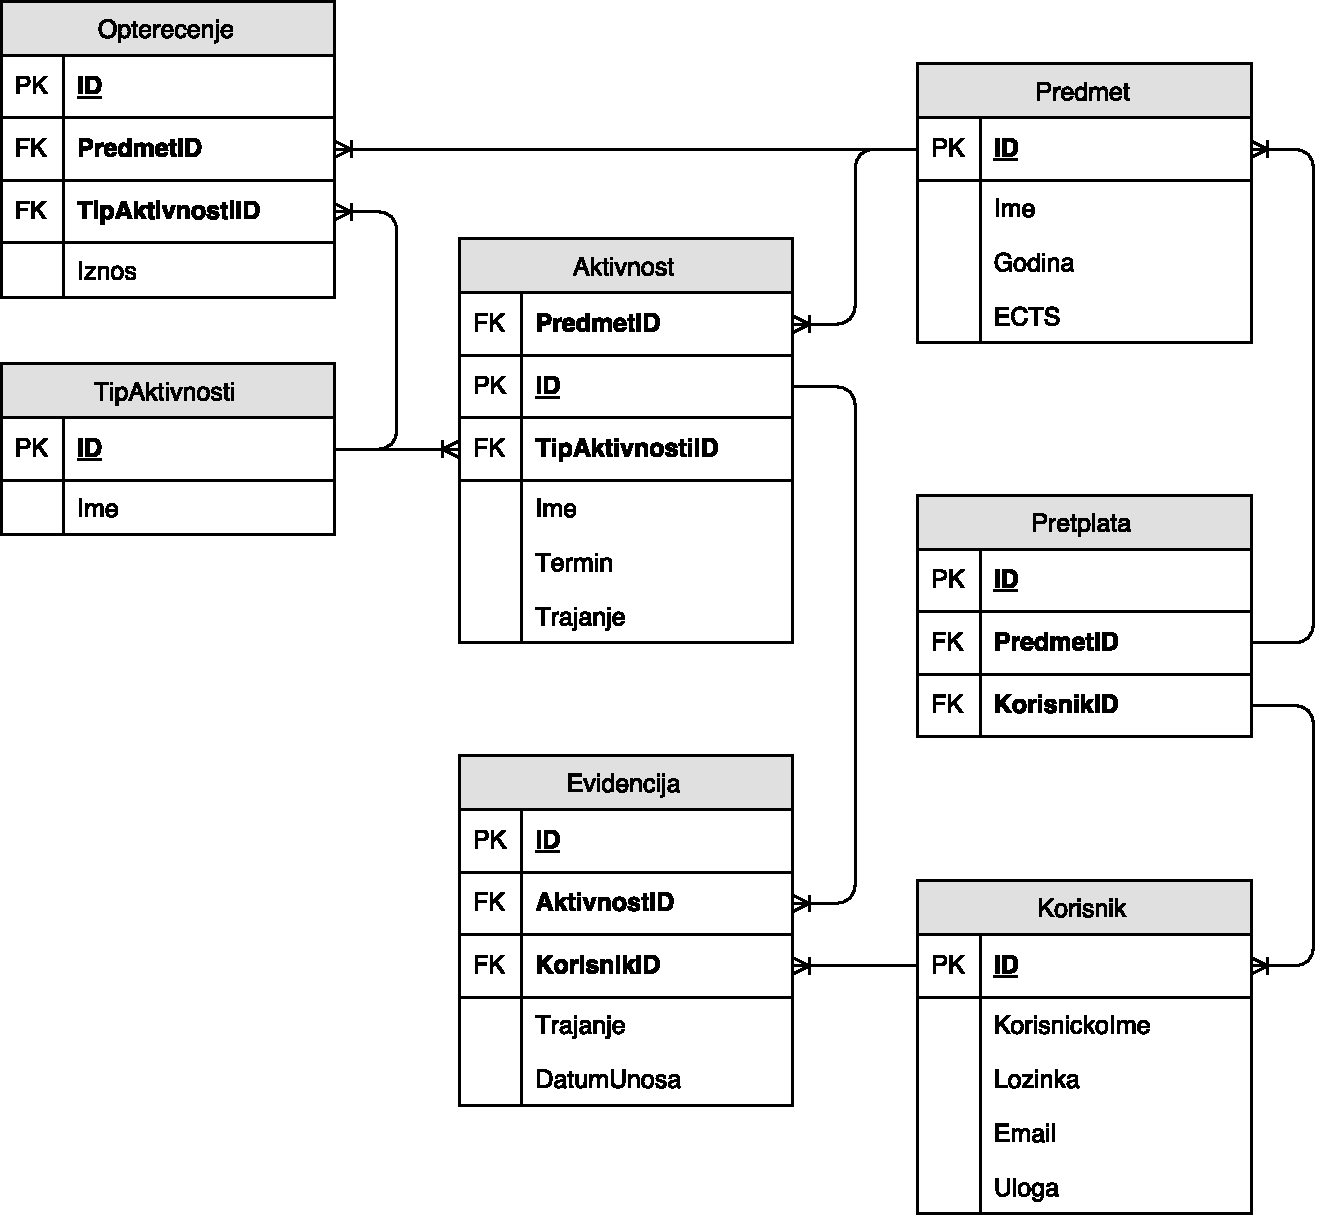
\includegraphics[scale=0.6]{img/relacijski-model.pdf}
\caption{Konačni ER model}
\label{fig:er-model}
\end{figure}

\section{Relacijski model}
\subsection{Dijagram}

\begin{figure}[H]
\centering
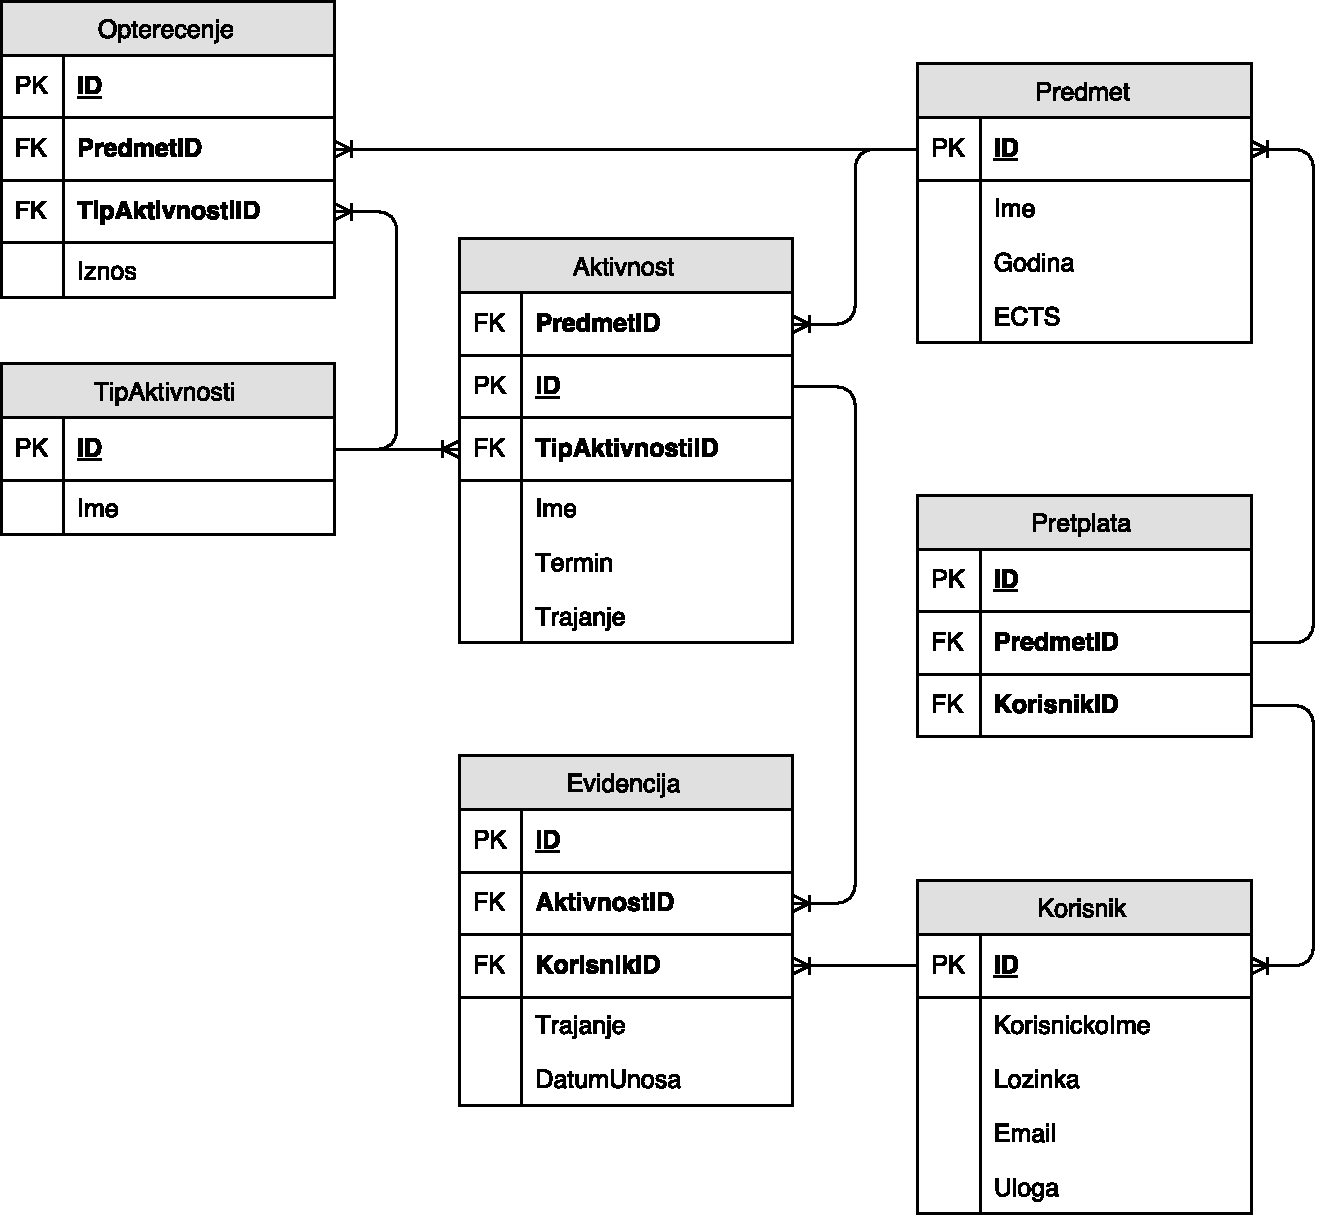
\includegraphics[scale=0.6]{img/relacijski-model.pdf}
\caption{Relacijski model}
\label{fig:relacijski-model}
\end{figure}

\subsection{SQL kod}
\lstset{style=sql}
\lstinputlisting{code/baza.sql}

\chapter{Web aplikacija}
\section{Alati i tehnologije}
\begin{enumerate}
\item \textbf{SQL Server Management Studio}
\item \textbf{SQL Server 2016}
\item \textbf{Entity Framework}
\item \textbf{ASP.NET}
\item \textbf{jQuery}
\item \textbf{AJAX}
\end{enumerate}

\section{Implementacija}
\subsection{Prijava}
Da bi korisnik uopće mogao koristiti bilo koji dio aplikacije, treba se prvo prijaviti u sustav putem korisničkog računa, kao što to obično jest u većini slučajeva kada god su u pitanju web aplikacije. Potrebo je implementirati barem najosnovniji dio sustava za prijavu, kako bi se sve evidencije mogle povezati sa svojim odgovarajućim korisnicima. Na ovaj način korisnik može tijekom pregleda statistike vidjeti zasebno svoju statistiku (izračunatu temeljem njegovih evidencija), a zasebno sve ostalo.

\begin{figure}[H]
\centering
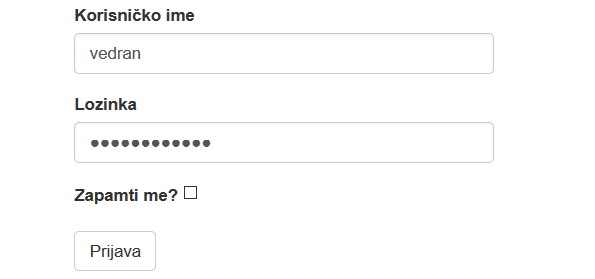
\includegraphics[width=\textwidth,height=\textheight,keepaspectratio]{img/prijava.png}
\caption{Prijava}
\label{fig:prijava}
\end{figure}

Stranica za prijavu sastoji se od polja za unos korisničkog imena i polja za unos lozinke, gdje korisnik upisuje svoje korisničke podatke. Nakon unosa podataka korisnik odabire tipku 'Prijava' čime se šalje zahtjev za autentifikaciju. Server tada uzima korisničko ime od klijenta te provjerava da li navedeni korisnik usitinu postoji u bazi podataka. Ako korisničko ime ne postoji, klijentu se ispisuje odgovarajuća greška. Ako postoji, to znači da u bazi postoji n-torka u relaciji 'Korisnik' koja sadrži sve korisnikove podatke, uključujući i njegovu kriptiranu lozinku. Lozinka koju je korisnik unio prilikom prijave sada se enkriptira te se uspoređuje sa lozinkom pohranjenom u bazi.

\lstset{style=csharp}
\lstinputlisting{code/prijava.cs}

Ako su jednake, autorizacija uspijeva te korisnik biva prijavljen, nakon čega ga se preusmjerava na stranicu za odabir predmeta. U slučaju pogreške ispisuje se odgovarajuća greška: nepostojeće korisničko ime, ili pogrešna lozinka.

Prilikom prijave moguće je označiti dodatnu opciju 'Zapamti me?'. Bez te opcije, nakon prijave, korisnik će nakon jedog vremenskog perioda neaktivnosti biti automatski odjavljen. Sa tom opcijom, serveru se daje do znanja da zapamti korisnika i da ga ne odjavi nakon navedenog vremenskog perioda, nega da ga zapamti dokle god se u 'kolačićima' klijentovih zahtjeva nalazi identifikator sjednice (engl. session id).

U slučaju da korisnik nema već postojeći račun na koji se može prijaviti, postoji i mogućnost registracije novog korisničkog računa:

\begin{figure}[H]
\centering
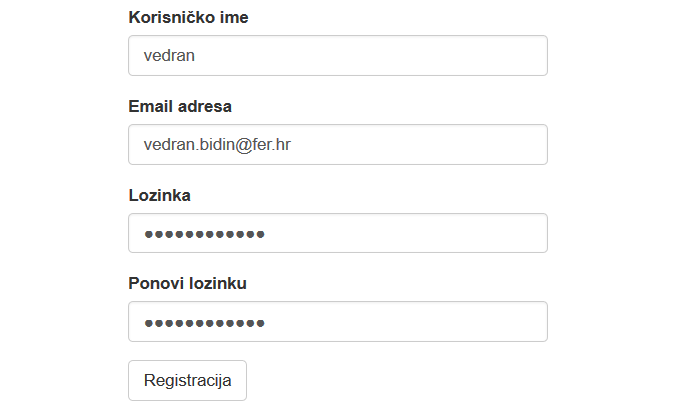
\includegraphics[width=\textwidth,height=\textheight,keepaspectratio]{img/registracija.png}
\caption{Registracija}
\label{fig:registracija}
\end{figure}

Kao što je vidljivo iz slike, potrebno je unesti osnovne podatke: korisničko ime, email adresu, te lozinku. U slučaju da navedeno korisničko ime već postoji u bazi, registracija neće biti moguća, pošto korisnička imenu moraju biti unikatna. Lozinku je potrebnu unesti dva puta, kako bi se smanjila mogućnost registracije sa pogrešno unesenom lozinkom.

Prijava i registracije oboje se provode koristeći klasični HTTP POST zahtjev, čija se obrada znatno olakšava korištenjem modela:
Model je obični razred koji sadrži neki broj polja, koja mogu biti bilo kojih tipova. Za svako polje mogu biti definirani određeni atributi, koji postavljaju dodatna ograničenja (da li polje nužno mora biti uneseno, da li mora sadržavati barem \textbf{N} broj znakova, i slično):

\lstset{style=csharp}
\lstinputlisting{code/registracija-model.cs}

Na početku pogleda (na prvoj liniji) deklarira se put do modela koji predstavlja sve podatke koji mogu biti unešeni:

\lstset{style=html}
\lstinputlisting{code/model.cshtml}

Tada se u pogledu definiraju elementi koji odgovaraju podacima iz modela. Za sve podatke koje je potrebno unesti, postavljaju se odgovarajući \textbf{input} elementi (koji mogu biti tekstovna polja, gumbi, padajuće liste i slično) koji služe za pohranu unesenih korisnikovih podataka te napokon \textbf{submit} tipka čijom pritiskom se šalje POST zahtjev. Svi elementi se dodatno enkapsuliraju sa \textbf{form} elementom, čime se podaci koji sadrže šalju u POST zahtjevu.

\lstset{style=html}
\lstinputlisting{code/registracija-view.cshtml}

Zatim se u kontroleru koji prima HTTP zahtjev kao jedan od parametara dodaje prethodno definirani model, čime se tijekom svake obrade HTTP zahtjeva može podacima iz forme na jednostavan način pristupiti preko parametra koji predtavlja taj model:

\lstset{style=csharp}
\lstinputlisting{code/registracija-cont.cs}

\subsection{Pretplata}
Nakon što je korisnik prijavljen, on može evidentirati te pregledavati svoje utrošeno vrijeme. Međutim, kako se sve evidencije zapravo vežu uz određeni predmet, evidentiranje i pregled se izvršavaju u odnosu na jedan od mnogih dostupnih predmeta. Zato korisnik uvijek prije evidencije odnosno pregleda mora odabrati jedan od tih predmeta. Kako broj predmeta može biti poprilično velik, korisnik bi prije svake evidencije i pregleda morao tražiti od svih mogućih predmeta onaj za koji želi evidentirati odnosno pregledavati statistiku. Zato je korisniku omogućena pretplata na predmet:

\begin{figure}[H]
\centering
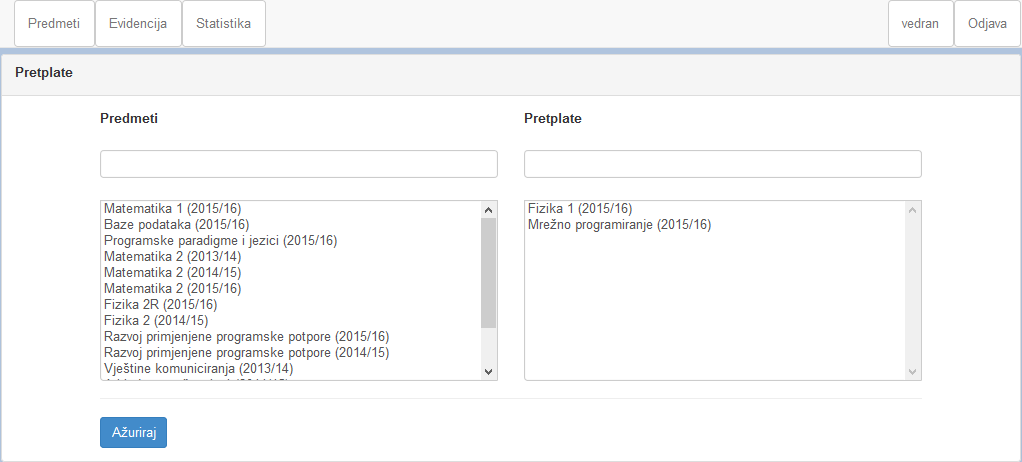
\includegraphics[width=\textwidth,height=\textheight,keepaspectratio]{img/pretplata-web.png}
\caption{Pretplata}
\label{fig:pretplata-web}
\end{figure}

U ovom dijelu trenutno prijavljeni korisnik može definirati na koje predmete želi biti pretplaćen. U lijevoj listi nalaze se svi dostupni predmeti, a u desnoj listi se nalaze svi pretplaćeni predmeti. Korisnik može selekcijom na bilo koje od predmeta ili bilo koje grupe predmeta dodavati odnosno brisati odgovarajuće pretplate. 

\textbf{Bootstrap Dual Listbox}\\
Popisi pretplaćenih i nepretplaćenih predmeta ostvareni su pomoću \textbf{Bootstrap Dual Listbox} plugin-a koji omogućava lagano upravljanje dvojnom listom. U pogledu za pretplate definira se \textbf{select} element, nad kojim se tijekom učitavanja stranice poziva funkcija \emph{bootstrapDualListbox()} sa pripadajućim opcijama:

\lstset{style=js}
\lstinputlisting{code/duallistbox.js}

Nakon svih izmjena, pritiskom na tipku 'Ažuriraj' provode se sve promjene te se ažurira popis pretplata odabrane od strane korisnika. Nakon toga u ostalim dijelovima web aplikacije korisnik na raspolaganju za odabir ima samo predmete na koje se unutar ove stranice pretplatio.

Ako se slanje novih pretplaćenih predmeta radi klasničnim POST zahtjevom, cijela stranica nakon ažuriranja se ponovno učitava, kako je to i inače slučaj sa običnim HTTP POST zahtjevima. Međutim, poželjno je ažurirati popis pretplaćenih predmeta bez ponovnog učitanja cijele stranice, jer to podrazumijeva ponovno čitanje \textbf{svih} predmeta iz baze podataka, što nepotrebno troši vrijeme servera, pošto su svi predmeti već bili učitani prilikom prvog otvaranja stranice.

Zato se slanje ažuriranih pretplata radi korištenjem \textbf{AJAX}-a. Definira se funkcija koja se poziva tijekom pritiska tipke 'Ažuriraj', koja prvo iz liste predmeta pronalazi sve one na koje je korisnik pretplaćen te ih sprema u polje koje sadrži njihove identifikatore. Zatim se koristi jQuery funkcija \emph{post()} (koja je omotač oko poziva funkcije \emph{ajax()}) koja prosljeđuje navedene identifikatore pretplaćenih predmeta serveru:

\lstset{style=js}
\lstinputlisting{code/pretplate-ajax.js}

Kontroler tada na osnovi dobivenih identifikatora, odnosno primarnih ključeva predmeta, ažurira korisnikove pretplaćene predmete.

Pošto broj predmeta može biti velik, dodatno na vrhu svakih od listi nalazi se polje za filtriranje. U to polje može se unesti niz znakova (dio ili cijeli naziv predmeta) nakon čega se lista odmah ažurira, te prikazuje samo one predmete koje sadrže navedeni niz znakova:

\begin{figure}[H]
\centering
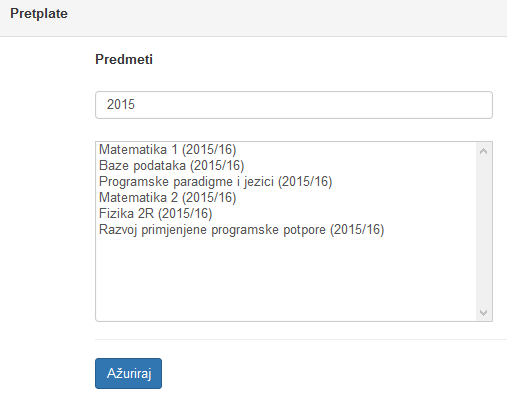
\includegraphics[width=\textwidth,height=\textheight,keepaspectratio]{img/filtriranje.png}
\caption{Filtriranje predmeta po godini}
\label{fig:filtriranje}
\end{figure}

\subsection{Evidencija}
Ovaj dio web aplikacije omogućava prijavljenim korisnicima da evidentiraju svoje utrošeno vrijeme za predmete na koje su pretplaćeni:

\begin{figure}[H]
\centering
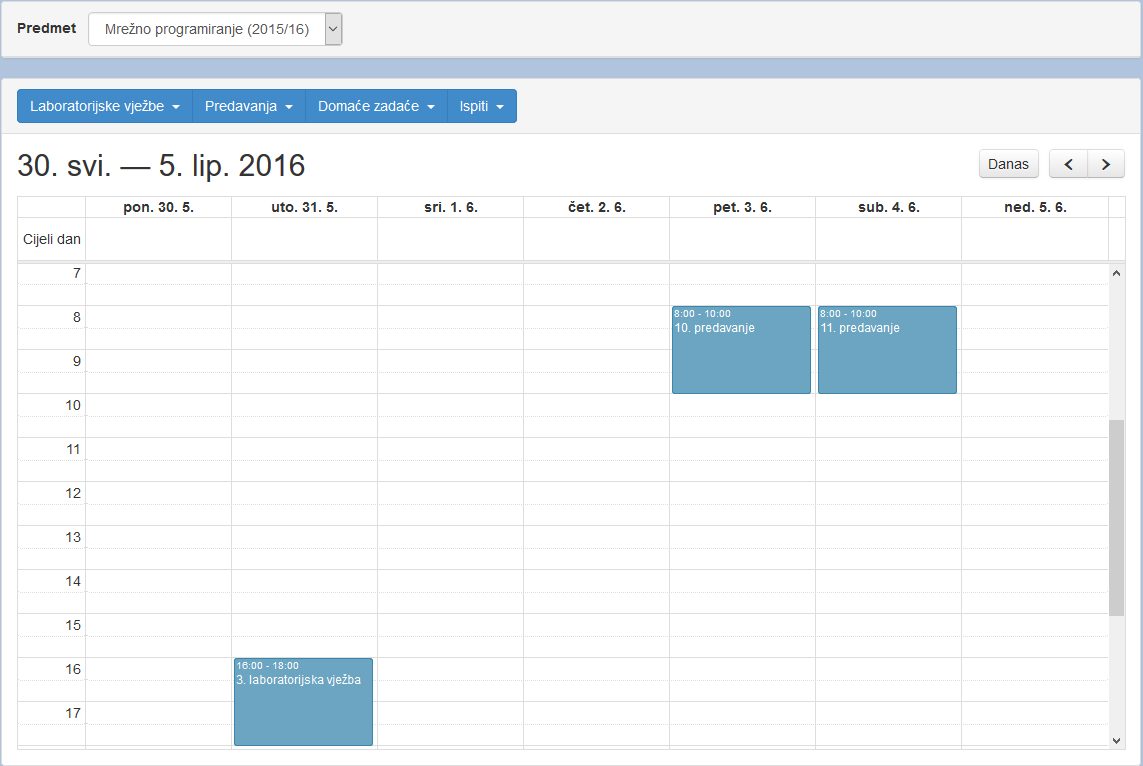
\includegraphics[width=\textwidth,height=\textheight,keepaspectratio]{img/evidencija-web.png}
\caption{Evidentiranje predmeta}
\label{fig:evidencija-web}
\end{figure}

Evidencija se sastoji od 3 dijela:

\begin{enumerate}
\item Na vrhu je padajuća lista koja sadrži sve pretplaćene predmete trenutno prijavljenog korisnika. Ovdje korisnik odabire predmet za koji želi evidentirati utrošeno vrijeme.

\item Izbornik aktivnosti. Nakon što korisnik odabere jedan od njegovih pretplaćenih predmeta putem padajuće liste, ovaj izbornik dinamički se ažurira sa svim novim aktivnostima toga predmeta. Aktivnosti su podijeljene prema tipu aktivnosti: odabirom jednog od tipova aktivnosti otvara se nova padajuća lista koja sadrži sve aktivnosti toga tipa. Naprimjer ako za predmet 'Mrežno programiranje' odaberemo tip aktivnosti 'Predavanja', stranica bi mogla izgledati ovako:

\begin{figure}[H]
\centering
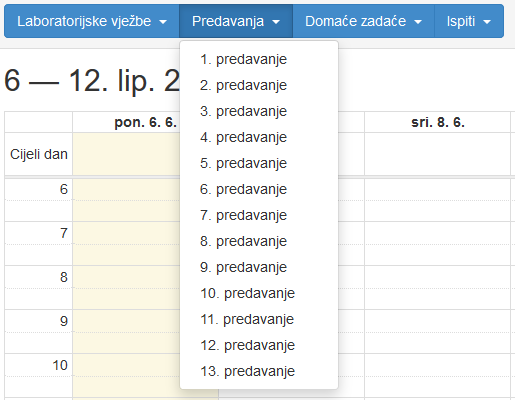
\includegraphics[width=\textwidth,height=\textheight,keepaspectratio]{img/selekcija.png}
\caption{Odabir tipa aktivnosti}
\label{fig:selekcija}
\end{figure}

Nakon što je odabran tip aktivnosti, korisnik ima pregled svih aktivnosti toga tipa, te tada odabire jednu od tih aktivnosti, onu za koju želi evidentirati utrošeno vrijeme. Nakon odabira aktivnosti otvara se novi modalni prozor:

\begin{figure}[H]
\centering

\includegraphics[width=\textwidth,height=\textheight,keepaspectratio]{img/modal.png}
\caption{Unos utrošenog vremena}
\label{fig:modal}
\end{figure}

Modalni prozor sastoji se od polja u koje se unosi iznos utrošenog vremena, i padajuće liste u kojoj se odabire mjerna jedinica utrošenog vremena (minute ili sati). Nakon što korisnik unese podatke, odabere se opcija spremi čime se vrši validacija. U slučaju pogreške unosa podataka, naprimjer ako se umjesto iznosa vremena unese riječ ili slično, korisniku se ispisuje odgovarajući tekst pogreške. Ako je validacija prošla, unos se trajno pohranjuje u bazu, nakon čega se kao i sve ostale pohranjene evidencije koristi prilikom računanja statistike koja je dostupna na stranici imena 'Statistika'. U slučaju pogreške od strane korisnika, modalni prozor može se ugasiti pritiskom na 'x' gumb u gornjem desnom kutu prozora čime se evidentiranje za tu specifičnu aktivnost otkazuje. Bez obzira na rezultat evidencije, korisnik opet može proizvoljno odabirati i evidentirati aktivnosti koliko god je potrebno.

\item Kalendar

TODO: dodaj sliku kalendara sa aktivnostima:

Osim prethodno navedenog načina evidentiranja (odabirom aktivnosti putem izbornika), korisniku se dodatno omogućuje i evidentiranje putem kalendara. Sve aktivnosti odabranoga predmeta koje imaju u bazi definiran datum početka i/ili trajanje, mogu se vidjeti na kalendaru, ukoliko su to aktivnosti trenutnog predmeta. Korisnik može pregledavati sve aktivnosti putem kalendara, te ih aktivirati pritiskom na njih. Nakon takvog odabira, opet se otvara isti modalni prozor kao i prilikom klasičnog evidentiranja koji korisniku omogućuje evidentiranje. Važno je za napomenuti da neke aktivnosti nemaju definiran datum početka. U tom slučaju te aktivnosti se očito nemogu aktivirati putem kalendara, već se moraju odabrati putem izbornika.
\end{enumerate}


\subsection{Statistika}
Ovaj dio web aplikacije omogućava prijavljenim korisnicima da pregledaju svoje trenutačno utrošeno vrijeme, te da ga uspoređuju sa drugim korisnicima kao i sa definiranim očekivanim utrošenim vremenom. Kao i kod drugih dijelova aplikacije, korisnik mora biti prijavljen na sustav. Nakon odabira stranice evidencija korisnik ima na raspolaganju dvije kartice, prva od kojih omogućuje sljedeći pregled:

\begin{figure}[H]
\centering
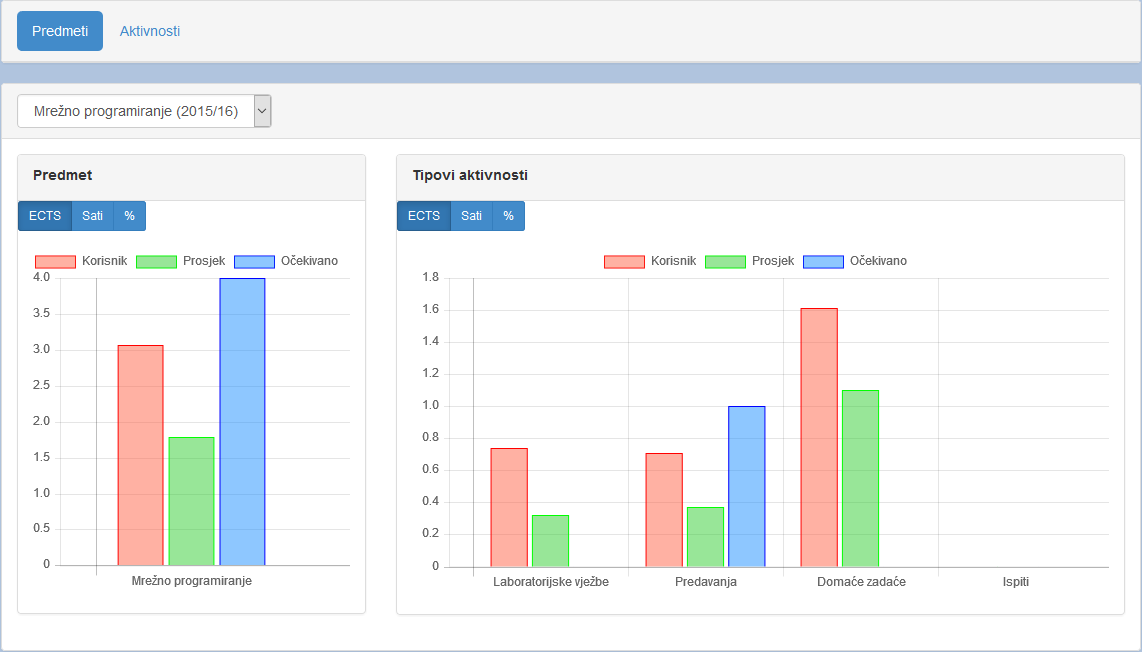
\includegraphics[width=\textwidth,height=\textheight,keepaspectratio]{img/statistika-web.png}
\caption{Statistika - kartica Predmeti}
\label{fig:statistika-web}
\end{figure}

Korisnik ovdje može odabrati jedan od predmeta na koje je trenutačno pretplaćen. U slučaju da predmet koji korisnik želi pregledavati nije na ovom popisu, potrebno je u izborniku 'Predmeti' pretplatiti se na taj predmet, nakon čega će on postati vidljiv u padajućoj listi.

Nakon odabira korisnika, odmah se ažurira statistika predmeta, tipova aktivnosti, te i samih aktivnosti. Korisnik ima na raspologanja 3 grafa. Prvi graf 'Predmet' omogućuje korisniku pregled utrošenog vremena na razini cijelog predmeta, odnosno obuhvaća ukupan iznos utrošenog vremena. Sve evidencije koje je korisnik ikada evidentirao za trenutačno navedeni predmet bit će pokazane u obliku stupičastog grafa u trenutno odabranim mjernim jedinicama. Osim samih korisnikovih podataka, također su i na raspolaganju drugi podaci: jedan od njih je prosjek utrošenog vremena svih evidencija za taj predmet. Pod time se zapravo misli na prosjek utrošenog vremena svih korisnika koji su ikada evidentirali ovaj predmet.

Osim tog podatka, također postoji i iznos ECTS bodova koji je definiran za svaki predmet prilikom njegovog unosa. Sa ECTS bodovima može se izračunati očekivani utrošak vremena za taj predmet, pošto se uzima da jedan ECTS bod iznosi ~28 sati. Korisnik može vidjeti koliko je vremena utrošio on, koliki je prosjek utrošenog vremena, te koliko je vremena 'trebalo' (otprilike) biti utrošeno. To je korisna informacija koja može pokazati koliko je dobro definiran predmet: da li uzima manje vremena nego što bi trebao, više nego što bi trebao, te u kojim iznosu prekoračuje očekivano vrijeme.

\begin{figure}[H]
\centering
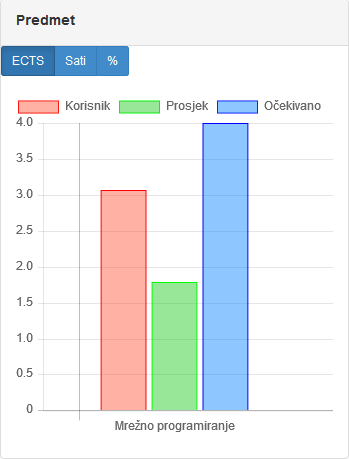
\includegraphics{img/statistika-predmet.png}
\caption{Statistika - predmet}
\label{fig:statistika-predmet}
\end{figure}

Osim pregleda ukupno utrošenog vremena, korisnik također može pregledavati utrošeno vrijeme po tipovima aktivnosti koji su definirani za trenutačno odabrani predmet. Naprimjer, ako korisnik odabere predmet 'Mrežno programiranje', mogli bismo vidjeti sljedeću sliku:

\begin{figure}[H]
\centering
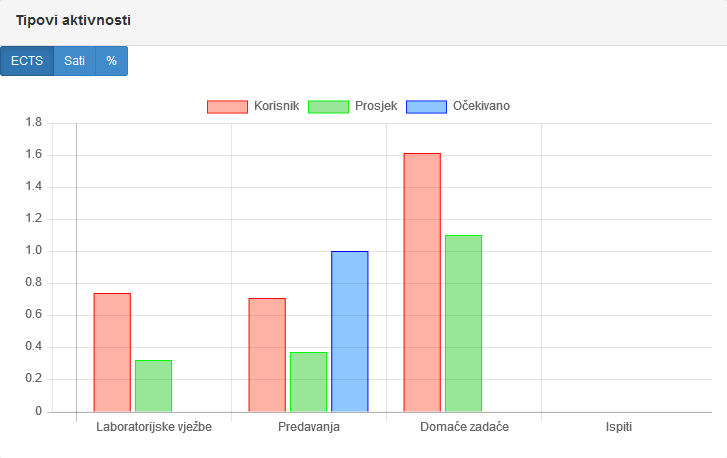
\includegraphics[width=\textwidth,height=\textheight,keepaspectratio]{img/statistika-tip-aktivnosti.png}
\caption{Statistika - tipovi aktivnosti}
\label{fig:statistika-tip-aktivnosti}
\end{figure}

Stupčasti graf sadrži iste 3 komponente kao i graf predmeta: iznos utrošenog vremena korisnika, prosječno utrošeno vrijeme, te očekivano utrošeno vrijeme (ukoliko postoji). Iznosi ovih komponenti definirani su za svaki tip aktivnosti trenutno odabranog predmeta. U slučaju tipa aktivnosti kao što su 'predavanja', u sklopu predmeta može biti definirano semestralno opterećenje sa određenim iznosom, koje određuje koliko vremena bi trebalo biti utrošeno za taj tip aktivnosti. To vrijeme se tada može direktno prikazati u grafu, čime se može vidjeti odstupanje od očekivane vrijednosti. Osim slučaja gdje je trajanje nekog tipa aktivnosti službeno definiran, očekivani utrošak vremena može se definirati 'ručno', za bilo koji tip aktivnosti, čime se može sustavu dati do znanja koliko bi vremena trebalo biti utrošeno za taj tip aktivnosti. Isto tako, moguće je da očekivano vrijeme ne postoji ili nije definirano, u kojem slučaju ono neće biti ni prikazano.

Ova statistika također prikazuje zanimljive podatke. Pregled utrošenog vremena po predmetu daje nam opći pogled na predmet, dok sa ovom statistikom ulazimo jedan sloj dublje: sada je dostupan pregled utrošenog vremena po tipu aktivnosti. Sa ovim pogledom možemo vidjeti na koji način je raspodijeljeno utrošeno vrijeme: da li premalo ljudi ide na predavanja, da li laboratorijske vježbe oduzimaju previše vremena, da li su domaće zadaće previše lagane i slično.

Još postoji i treći graf: iznos utrošenog vremena po aktivnostima. Kada se odabere drugi izbornik, sučelje izgleda otprilike kao na slici:

\begin{figure}[H]
\centering
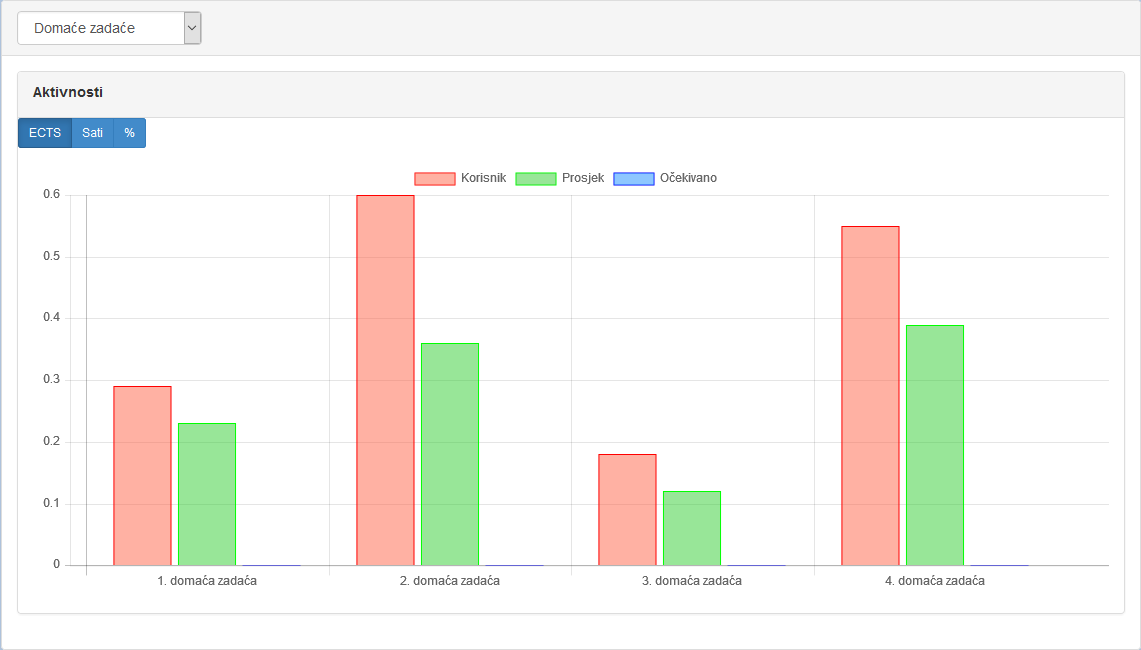
\includegraphics[width=\textwidth,height=\textheight,keepaspectratio]{img/statistika-aktivnosti.png}
\caption{Statistika - aktivnosti}
\label{fig:statistika-aktivnosti}
\end{figure}

Kao i na prijašnjoj kartici, na vrhu se nalazi padajuća lista. Međutim, sada padajuća lista sadrži sve tipove aktivnosti, i to sve tipove aktivnosti trenutačno odabranog predmeta na kartici 'Predmet'. Nakon odabira novog predmeta na prethodnoj kartici, ova padajuća lista odmah se osvježava, sa novim vrijednostima koje odgovaraju odabranom predmetu. Korisnik može izabrati jedan od ponuđenih tipova aktivnosti. Prilikom izbora novog tipa aktivnosti, dohvaćaju se sve aktivnosti koje su tog tipa, i koje pripadaju prethodno odabranome predmetu, zajedno sa svim njihovim evidencijama, te se grafički predočuje iznos utrošenog vremena po specifičnoj aktivnosti. Sa ovim grafom najdetaljnije se predočuje utrošeno vrijeme: može se vidjeti točno koliko je vremena utrošeno na pojedinačnu aktivnost što isto može biti korisna informacija.

Naprimjer, ako se pregledavaju sve laboratorijske vježbe određenoga predmeta, može se vidjeti koliko je vremena utrošena na jednu laboratorijsku vježbu, što je već samo po sebi dovoljan razlog za pregled ovog grafa. Međutim također se može vidjeti koliko je vremena utrošeno na specifičnu laboratorijsku vježbu (odnosno bilo koju aktivnost) u odnosu na druge aktivnosti. Time se može naprimjer uočiti da je određena laboratorijska vježba oduzela premalo vremena s obzirom na druge laboratorijske vježbe, ili da je priprema za laboratorijsku vježbu preteška s obzirom na samu laboratorijsku vježbu ili na druge pripreme.

Osim samog iznosa utrošenog vremena za korisnika i za prosjek, za svaku aktivnost u bazi podataka može biti evidentirano trajanje te aktivnosti. U slučaju primjerice predavanja to trajanje doslovce predstavlja predefinirani iznos trajanja predavanja određenog termina kao što je određeno po predmetu. Međutim, za aktivnosti koji nemaju već strogo definirana trajanja moguće je prilikom unosa aktivnosti definirati 'očekivano' trajanje, koje korisnicima daje do znanja koliko je vremena otprilike trebalo biti potrebno, ili koliki je očekivani utrošak vremena za tu aktivnost. U svakom slučaju, ako ta vrijednost nije poznata, ili čak nije ni važna, nije ju potrebnu ni unesti, pa će ta vrijednost tada ovdje biti neprikazana.

\subsection{Unos podataka}

TODO

\section{Razvoj i poboljšanje}

TODO

\chapter{Zaključak}
TODO

\bibliographystyle{fer}
\bibliography{literatura}

\begin{sazetak}
Sažetak na hrvatskom jeziku.

\kljucnerijeci{Ključne riječi, odvojene zarezima.}
\end{sazetak}

% TODO: Navedite naslov na engleskom jeziku.
\engtitle{Title}
\begin{abstract}
Abstract.

\keywords{Keywords.}
\end{abstract}

\end{document}
